% \documentclass[conference]{IEEEtran}
% \IEEEoverridecommandlockouts
% % The preceding line is only needed to identify funding in the first footnote. If that is unneeded, please comment it out.
% \usepackage{cite}
% \usepackage{amsmath,amssymb,amsfonts}
% \usepackage{algorithmic}
% \usepackage{graphicx}
% \usepackage{textcomp}
% \usepackage{xcolor}
% \usepackage{enumerate}
% \usepackage{booktabs}
% \usepackage{float}
% \usepackage{hyperref}
% \usepackage{subfigure}
% \usepackage{subcaption}
% \def\BibTeX{{\rm B\kern-.05em{\sc i\kern-.025em b}\kern-.08em
%     T\kern-.1667em\lower.7ex\hbox{E}\kern-.125emX}}
% \begin{document}

% \title{Evaluating and Improving Chunking Methods for Search and Retrieval-Augmented Generation (RAG) Systems\\
% }
% \author{\IEEEauthorblockN{Shelly Schwartz}
% \IEEEauthorblockA{\textit{University of Virginia} \\
% \textit{School of Data Science}\\
% Charlottesville, Virginia \\
% tfk6ua@virginia.edu}
% }

% \maketitle

% \begin{abstract}
% Chunking, the process of segmenting long documents into coherent and semantically independent units, is a foundational step in retrieval-based systems and Retrieval-Augmented Generation (RAG) pipelines. Existing approaches often use fixed-size segmentation or sentence heuristics that fail to capture semantic boundaries, producing incoherent or redundant text segments that reduce retrieval precision and degrade the quality of generated answers. This work aims to reproduce several recent chunking algorithms, benchmark their strengths and weaknesses under a unified evaluation framework, and propose improved intrinsic evaluation methods based on dynamic programming optimization and LLM-as-a-Judge scoring.
% \end{abstract}

% \begin{IEEEkeywords}
% Chunking, Search, Retrieval-Augmented Generation, RAG, Intrinsic Evaluation, Dynamic Programming, LLM-as-a-Judge
% \end{IEEEkeywords}

% \section{Introduction}
% Chunking determines how information is represented and retrieved in both search and RAG pipelines. When documents are split into poorly defined segments, retrievers cannot retrieve relevant text consistently, and generation models may hallucinate or lose factual grounding. Effective chunking should maintain logical continuity, avoid redundancy, and ensure that each chunk represents a complete semantic unit. However, most current chunking techniques emphasize simplicity or computational efficiency over linguistic or semantic integrity.

% Existing methods present several downsides:
% \begin{itemize}
%     \item \textbf{Fixed-size windowing} (common in baseline retrievers) ignores semantic boundaries, leading to arbitrary splits that fragment meaning and break logical flow.
%     \item \textbf{Sentence-based segmentation} performs inconsistently because sentences vary greatly in length and informational density. Short sentences produce under-informative chunks, while long sentences may combine multiple ideas into a single unit.
%     \item \textbf{Late Chunking}~\cite{gunther2024late} preserves global context by chunking after encoding, but it lacks redundancy control. Similar information can appear in multiple chunks, increasing index size and retrieval noise.
%     \item \textbf{CrossFormer}~\cite{ni2025crossformer} approaches chunking as a supervised segmentation problem. It introduces a Cross-Segment Fusion Module (CSFM) that learns token-level attention transitions to identify meaningful boundaries.
%     \item \textbf{S2 Chunking}~\cite{verma2025s2chunking} combines structural and semantic information, leveraging layout cues such as headings, bullet lists, and table structures alongside embedding similarity.
%     \item \textbf{HiChunk}~\cite{lu2025hichunk} captures hierarchical structures but remains computationally expensive and reliant on large annotated datasets.
%     \item \textbf{HOPE}~\cite{bradland2025hope} provides automatic intrinsic evaluation, yet its reliance on embedding models introduces potential bias and instability.
% \end{itemize}

% The goal of this project is twofold: first, to reproduce and rigorously evaluate these chunking algorithms under consistent experimental conditions, and second, to propose two novel approaches for more accurate and interpretable segmentation.

% \subsection{Limitations of Typical Evaluation Methods}
% Chunking quality is typically measured indirectly through retrieval performance metrics such as nDCG@10, Recall@K, and MRR, as implemented in BEIR~\cite{thakur2021beir}. Improvements in these values are often interpreted as evidence of better chunking. However, this assumption is flawed because retrieval performance depends on multiple factors unrelated to segmentation quality, including retriever architecture, embedding dimensionality, and ranking models.

% Moreover, many chunking evaluations rely on simplistic or heuristic proxies:
% \begin{itemize}
%   \item \textbf{Retrieval-only metrics:} Treat chunking success as equivalent to higher retrieval precision, ignoring semantic coherence.
%   \item \textbf{Answer-span overlap:} Evaluate chunking by how often chunks contain QA answer spans (e.g., SciFact~\cite{wadden2020scifact}), which rewards short localized evidence but not meaningful segmentation.
%   \item \textbf{Boundary alignment:} Compare predicted splits with sentence or paragraph breaks without assessing semantic independence.
% \end{itemize}

% These methods fail to capture intrinsic chunking quality. A good segmentation should ensure that chunks are both self-contained and non-redundant, properties that standard retrieval metrics do not measure. Hence, we propose evaluation frameworks that quantify these properties directly.

% \section{Literature Review}
% \subsection{Late Chunking (G{\"u}nther et al., 2024)}
% Late Chunking~\cite{gunther2024late} introduces post-transformer segmentation, where full-document embeddings are generated before chunking. Each chunk embedding incorporates context from the entire document, leading to better representation of long dependencies. Although this approach yields consistent improvements on BEIR datasets such as SciFact, FiQA, and TREC-COVID, it increases computational cost and fails to penalize redundant chunks that represent similar meanings.

% \subsection{CrossFormer (Ni et al., 2025)}
% CrossFormer~\cite{ni2025crossformer} approaches chunking as a supervised segmentation problem. It introduces a Cross-Segment Fusion Module (CSFM) that learns token-level attention transitions to identify meaningful boundaries. This model yields smoother inter-chunk transitions and improved retrieval accuracy but requires large labeled datasets and may overfit to specific text distributions, reducing generalization.

% \subsection{S2 Chunking (Verma et al., 2025)}
% S2 Chunking~\cite{verma2025s2chunking} combines structural and semantic information, leveraging layout cues such as headings, bullet lists, and table structures alongside embedding similarity. The approach performs well on semi-structured documents but is less effective on unstructured text. Its reliance on formatting metadata limits adoption in domains without clear document structure.

% \subsection{HiChunk (Lu et al., 2025)}
% HiChunk~\cite{lu2025hichunk} models hierarchical relationships between sections, paragraphs, and sentences, allowing multi-scale segmentation. Its HiCBench dataset provides annotated boundaries at different granularities. Although this enables hierarchical evaluation, it demands intensive annotation and computational resources.

% \subsection{HOPE (Br{\aa}dland et al., 2025)}
% HOPE~\cite{bradland2025hope} proposes one of the first intrinsic evaluation frameworks for chunking, quantifying cohesion, task utility, and coherence automatically using embedding-based statistics. However, it depends on the underlying embedding model, meaning performance varies across architectures. Despite this limitation, HOPE sets an important precedent for intrinsic chunk evaluation.

% \subsection{Synthesis of Current Research}
% Across all methods, there is a clear tension between structural fidelity and semantic coherence. Approaches that emphasize structure, such as S2 Chunking and HiChunk, preserve formatting but neglect contextual embedding relationships. In contrast, embedding-based methods like Late Chunking and CrossFormer maximize semantic continuity but risk redundancy and computational inefficiency. These trade-offs highlight the need for hybrid or adaptive chunking strategies that combine structure-aware and semantic optimization.

% \section{Proposed Method}
% We propose two complementary approaches for chunking that address the weaknesses of existing methods. The first method formulates chunking as a dynamic programming (DP) optimization problem that explicitly balances intra-chunk cohesion and inter-chunk separation. The second method applies recursive splitting guided by structural and token-level similarity signals to produce logically coherent segments.

% \subsection{Method 1: Dynamic Programming for Cohesion and Separation}
% This method defines an optimization objective over embedding blocks. Let $E_i$ be the embedding of the $i$-th block of tokens. The best segmentation up to block $i$ is computed as:
% \[
%  dp[i] = \max_{j < i} \big[ dp[j] + w_c \cdot Cohesion(j,i) - w_s \cdot Separation(j,i) - \lambda \big]
% \]
% where:
% \begin{itemize}
%   \item $Cohesion(j,i)$ measures average cosine similarity among embeddings within $[j,i)$.
%   \item $Separation(j,i)$ penalizes similarity between the centroid of $[j,i)$ and centroids of previous chunks.
%   \item $\lambda$ is a fixed cost per split, preventing over-segmentation.
%   \item $w_c$ and $w_s$ weight cohesion and separation respectively.
% \end{itemize}
% To limit complexity, a beam search heuristic considers only the top $k$ split points at each step, reducing runtime from $O(N^2)$ to $O(kN)$. The algorithm returns chunk boundaries that maximize global coherence while minimizing redundancy. This DP framework makes segmentation an explicit optimization process, not a heuristic one.

% \subsection{Method 2: Recursive Structural Chunking}
% This approach uses both token-level similarity and document structure to identify natural boundaries. The algorithm operates as follows:
% \begin{enumerate}
%   \item Compute contextual embeddings for all tokens in the document.
%   \item Compute pairwise cosine similarities between adjacent tokens to detect discontinuities.
%   \item Assign each potential boundary a score based on a weighted combination of similarity gradients, whitespace signals, and structural cues (paragraphs, headers, lists, etc.).
%   \item Recursively split at the highest-scoring boundaries until chunk length or similarity constraints are met.
%   \item Apply an optional DP refinement to remove weak boundaries and merge semantically connected chunks.
% \end{enumerate}
% This recursive method adapts to both linguistic and structural changes in text. By leveraging paragraph and token-level cues, it preserves natural discourse flow while ensuring each segment represents a coherent semantic unit.

% \section{Dataset}
% \subsection{Dataset Overview}
% We evaluate chunking methods on four datasets commonly used in the BEIR benchmark suite~\cite{thakur2021beir}. These datasets span scientific, biomedical, finance, and pandemic-focused corpora, and each provides query--document relevance judgments that enable standard retrieval evaluation as well as chunking-specific analyses using positive/negative document labels.

% \begin{itemize}
%     \item \textbf{SciFact} consists of expert-written scientific claims paired with evidence-containing abstracts, supporting claim verification-style retrieval~\cite{wadden2020scifact}. We use the BEIR-formatted version for retrieval evaluation~\cite{thakur2021beir,beir_scifact_hf}. \textit{Link:} \url{https://huggingface.co/datasets/BeIR/scifact}~\cite{beir_scifact_hf}.
%     \item \textbf{NFCorpus} is a medical information retrieval dataset built from nutrition-related lay queries and PubMed-style documents~\cite{boteva2016nfcorpus}. We use the BEIR-formatted version for retrieval evaluation~\cite{thakur2021beir,beir_nfcorpus_hf}. \textit{Link:} \url{https://huggingface.co/datasets/BeIR/nfcorpus}~\cite{beir_nfcorpus_hf}. (Dataset reference page: \url{https://ir-datasets.com/nfcorpus.html}~\cite{irdatasets_nfcorpus}.)
%     \item \textbf{FiQA2018} is a finance-domain question answering dataset used to evaluate answer generation grounded in retrieved financial texts, and is frequently used as a retrieval+QA benchmark in BEIR-style evaluations~\cite{thakur2021beir,fiqa2018_site}. \textit{Link:} \url{https://sites.google.com/view/fiqa/home}~\cite{fiqa2018_site}.
%     \item \textbf{TREC-COVID} is a COVID-19 scientific literature retrieval challenge dataset constructed over CORD-19, with 50 topics and relevance judgments collected across multiple rounds~\cite{roberts2021treccovid}. \textit{Link:} \url{https://arxiv.org/abs/2104.09632}~\cite{roberts2021treccovid}.
% \end{itemize}

% \subsection{How We Use These Datasets for Chunking Evaluation}
% We use these datasets in two complementary ways:
% \begin{enumerate}
%     \item \textbf{Standard retrieval evaluation (extrinsic):} Because each dataset includes relevance labels (i.e., positive and negative query--document pairs), we can measure downstream retrieval performance (e.g., nDCG@10, Recall@K, MRR) under different chunking strategies, following BEIR-style evaluation protocols~\cite{thakur2021beir}.
%     \item \textbf{Intrinsic chunk-boundary evaluation (LLM-as-a-Judge):} In addition to retrieval metrics, we evaluate chunk boundary quality directly by sampling documents and scoring proposed segmentation boundaries with an LLM-as-a-Judge rubric (e.g., coherence, completeness, and topical purity). This isolates chunking quality from retriever idiosyncrasies and complements relevance-based evaluation.
% \end{enumerate}


% \section{Experiments}
% \subsection{Extrinsic Evaluation}
% Both methods will be evaluated using BEIR datasets~\cite{thakur2021beir}, including SciFact~\cite{wadden2020scifact}, FiQA2018~\cite{fiqa2018_site}, NFCorpus~\cite{boteva2016nfcorpus}, and TREC-COVID~\cite{roberts2021treccovid}. Retrieval metrics (nDCG@10, Recall@K, MRR) will assess how chunking affects retrieval relevance and ranking. Significance testing using paired t-tests will compare our results to those of reproduced baselines.

% \subsection{Intrinsic Evaluation with GPT-4 as a Judge}
% We will perform intrinsic chunk evaluation using GPT-4 as the primary evaluator within an LLM-as-a-Judge framework, following the guidelines of JudgeBench~\cite{tan2024judgebench} and ConsJudge~\cite{liu2025consjudge}. GPT-4 will be prompted to assess chunk boundaries on three axes: (1) \textit{Coherence} — whether each split divides semantically independent ideas; (2) \textit{Completeness} — whether each chunk forms a self-contained, contextually complete unit; and (3) \textit{Relevance Purity} — whether the content within a chunk maintains topical consistency without mixing unrelated information.

% Each boundary will receive ordinal scores ranging from 0 to 3 on each axis, with a macro-average defining overall boundary quality. To ensure robustness, the same scoring protocol will be compared across multiple chunking mechanisms including fixed-size windowing, Late Chunking~\cite{gunther2024late}, CrossFormer~\cite{ni2025crossformer}, S2 Chunking~\cite{verma2025s2chunking}, and the proposed dynamic programming and recursive structural approaches.

% Boundary quality distributions and pairwise comparisons will be analyzed to determine which methods yield the most coherent and independent segmentations. The evaluation will quantify inter-model consistency using multiple GPT-4 runs with prompt ensembling and temperature control. For validation, a subset of 200 samples will also be double-annotated by human evaluators to verify GPT-4 alignment. Results will highlight how intrinsic chunk quality correlates with retrieval performance across datasets.

% \section{Results}
% This section will report (1) extrinsic retrieval metrics across BEIR benchmarks and (2) intrinsic boundary-quality metrics from GPT-4 scoring. We will present comparisons between baseline fixed-size chunking, Late Chunking~\cite{gunther2024late}, CrossFormer~\cite{ni2025crossformer}, S2 Chunking~\cite{verma2025s2chunking}, HiChunk~\cite{lu2025hichunk}, HOPE~\cite{bradland2025hope}, and our proposed methods, including ablations over hyperparameters ($\lambda, w_c, w_s, k$) and stopping criteria for recursive splitting.

% \section{Conclusion}
% This project bridges the gap between heuristic segmentation and semantic optimization in chunking research. By reproducing and extending state-of-the-art methods, it provides a comprehensive benchmark integrating extrinsic retrieval performance and intrinsic chunk quality. The proposed dynamic programming and recursive structural chunking methods explicitly target semantic cohesion, semantic separation, and redundancy control, offering more interpretable and controllable segmentation than common heuristics. We expect these contributions to improve retrieval precision and downstream RAG answer fidelity across diverse domains.

% \bibliography{refs}
% \bibliographystyle{unsrt}

% \appendix

% \section{Appendix}
% Additional tables and figures for full ablation results, prompt templates for GPT-4 judging, and implementation details for DP beam search and recursive splitting will be included here.

% \end{document}


% \documentclass[conference]{IEEEtran}
% \IEEEoverridecommandlockouts
% % The preceding line is only needed to identify funding in the first footnote. If that is unneeded, please comment it out.
% \usepackage{cite}
% \usepackage{amsmath,amssymb,amsfonts}
% \usepackage{algorithmic}
% \usepackage{graphicx}
% \usepackage{textcomp}
% \usepackage{xcolor}
% \usepackage{enumerate}
% \usepackage{booktabs}
% \usepackage{float}
% \usepackage{hyperref}
% \usepackage{subfigure}
% \usepackage{subcaption}
% \def\BibTeX{{\rm B\kern-.05em{\sc i\kern-.025em b}\kern-.08em
%     T\kern-.1667em\lower.7ex\hbox{E}\kern-.125emX}}
% \begin{document}

% \title{Evaluating and Improving Chunking Methods for Search and Retrieval-Augmented Generation (RAG) Systems\\
% }
% \author{\IEEEauthorblockN{Shelly Schwartz}
% \IEEEauthorblockA{\textit{University of Virginia} \\
% \textit{School of Data Science}\\
% Charlottesville, Virginia \\
% tfk6ua@virginia.edu}
% }

% \maketitle

% \begin{abstract}
% Chunking, the process of segmenting long documents into coherent and semantically independent units, is a foundational step in retrieval-based systems and Retrieval-Augmented Generation (RAG) pipelines. Existing approaches often use fixed-size segmentation or sentence heuristics that fail to capture semantic boundaries, producing incoherent or redundant text segments that reduce retrieval precision and degrade the quality of generated answers. This work aims to reproduce several recent chunking algorithms, benchmark their strengths and weaknesses under a unified evaluation framework, and propose improved intrinsic evaluation methods based on dynamic programming optimization and LLM-as-a-Judge scoring.
% \end{abstract}

% \begin{IEEEkeywords}
% Chunking, Search, Retrieval-Augmented Generation, RAG, Intrinsic Evaluation, Dynamic Programming, LLM-as-a-Judge
% \end{IEEEkeywords}

% \section{Introduction}
% Chunking determines how information is represented and retrieved in both search and RAG pipelines. When documents are split into poorly defined segments, retrievers cannot retrieve relevant text consistently, and generation models may hallucinate or lose factual grounding. Effective chunking should maintain logical continuity, avoid redundancy, and ensure that each chunk represents a complete semantic unit. However, most current chunking techniques emphasize simplicity or computational efficiency over linguistic or semantic integrity.

% Existing methods present several downsides:
% \begin{itemize}
%     \item \textbf{Fixed-size windowing} (common in baseline retrievers) ignores semantic boundaries, leading to arbitrary splits that fragment meaning and break logical flow.
%     \item \textbf{Sentence-based segmentation} performs inconsistently because sentences vary greatly in length and informational density. Short sentences produce under-informative chunks, while long sentences may combine multiple ideas into a single unit.
%     \item \textbf{Late Chunking}~\cite{gunther2024late} preserves global context by chunking after encoding, but it lacks redundancy control. Similar information can appear in multiple chunks, increasing index size and retrieval noise.
%     \item \textbf{CrossFormer}~\cite{ni2025crossformer} approaches chunking as a supervised segmentation problem. It introduces a Cross-Segment Fusion Module (CSFM) that learns token-level attention transitions to identify meaningful boundaries.
%     \item \textbf{S2 Chunking}~\cite{verma2025s2chunking} combines structural and semantic information, leveraging layout cues such as headings, bullet lists, and table structures alongside embedding similarity.
%     \item \textbf{HiChunk}~\cite{lu2025hichunk} captures hierarchical structures but remains computationally expensive and reliant on large annotated datasets.
%     \item \textbf{HOPE}~\cite{bradland2025hope} provides automatic intrinsic evaluation, yet its reliance on embedding models introduces potential bias and instability.
% \end{itemize}

% The goal of this project is twofold: first, to reproduce and rigorously evaluate these chunking algorithms under consistent experimental conditions, and second, to propose two novel approaches for more accurate and interpretable segmentation.

% \subsection{Limitations of Typical Evaluation Methods}
% Chunking quality is typically measured indirectly through retrieval performance metrics such as nDCG@10, Recall@K, and MRR, as implemented in BEIR~\cite{thakur2021beir}. Improvements in these values are often interpreted as evidence of better chunking. However, this assumption is flawed because retrieval performance depends on multiple factors unrelated to segmentation quality, including retriever architecture, embedding dimensionality, and ranking models.

% Moreover, many chunking evaluations rely on simplistic or heuristic proxies:
% \begin{itemize}
%   \item \textbf{Retrieval-only metrics:} Treat chunking success as equivalent to higher retrieval precision, ignoring semantic coherence.
%   \item \textbf{Answer-span overlap:} Evaluate chunking by how often chunks contain QA answer spans (e.g., SciFact~\cite{wadden2020scifact}), which rewards short localized evidence but not meaningful segmentation.
%   \item \textbf{Boundary alignment:} Compare predicted splits with sentence or paragraph breaks without assessing semantic independence.
% \end{itemize}

% These methods fail to capture intrinsic chunking quality. A good segmentation should ensure that chunks are both self-contained and non-redundant, properties that standard retrieval metrics do not measure. Hence, we propose evaluation frameworks that quantify these properties directly.

% \section{Literature Review}
% \subsection{Late Chunking (G{\"u}nther et al., 2024)}
% Late Chunking~\cite{gunther2024late} introduces post-transformer segmentation, where full-document embeddings are generated before chunking. Each chunk embedding incorporates context from the entire document, leading to better representation of long dependencies. Although this approach yields consistent improvements on BEIR datasets such as SciFact, FiQA, and TREC-COVID, it increases computational cost and fails to penalize redundant chunks that represent similar meanings.

% \subsection{CrossFormer (Ni et al., 2025)}
% CrossFormer~\cite{ni2025crossformer} approaches chunking as a supervised segmentation problem. It introduces a Cross-Segment Fusion Module (CSFM) that learns token-level attention transitions to identify meaningful boundaries. This model yields smoother inter-chunk transitions and improved retrieval accuracy but requires large labeled datasets and may overfit to specific text distributions, reducing generalization.

% \subsection{S2 Chunking (Verma et al., 2025)}
% S2 Chunking~\cite{verma2025s2chunking} combines structural and semantic information, leveraging layout cues such as headings, bullet lists, and table structures alongside embedding similarity. The approach performs well on semi-structured documents but is less effective on unstructured text. Its reliance on formatting metadata limits adoption in domains without clear document structure.

% \subsection{HiChunk (Lu et al., 2025)}
% HiChunk~\cite{lu2025hichunk} models hierarchical relationships between sections, paragraphs, and sentences, allowing multi-scale segmentation. Its HiCBench dataset provides annotated boundaries at different granularities. Although this enables hierarchical evaluation, it demands intensive annotation and computational resources.

% \subsection{HOPE (Br{\aa}dland et al., 2025)}
% HOPE~\cite{bradland2025hope} proposes one of the first intrinsic evaluation frameworks for chunking, quantifying cohesion, task utility, and coherence automatically using embedding-based statistics. However, it depends on the underlying embedding model, meaning performance varies across architectures. Despite this limitation, HOPE sets an important precedent for intrinsic chunk evaluation.

% \subsection{Synthesis of Current Research}
% Across all methods, there is a clear tension between structural fidelity and semantic coherence. Approaches that emphasize structure, such as S2 Chunking and HiChunk, preserve formatting but neglect contextual embedding relationships. In contrast, embedding-based methods like Late Chunking and CrossFormer maximize semantic continuity but risk redundancy and computational inefficiency. These trade-offs highlight the need for hybrid or adaptive chunking strategies that combine structure-aware and semantic optimization.

% \section{Proposed Method}
% We propose two complementary approaches for chunking that address the weaknesses of existing methods. The first method formulates chunking as a dynamic programming optimization problem that explicitly balances intra-chunk cohesion and inter-chunk separation. The second method applies recursive splitting guided by structural and token-level similarity signals to produce logically coherent segments.

% \subsection{Method 1: Dynamic Programming for Cohesion and Separation}
% This method defines an optimization objective over embedding blocks. Let $E_i$ be the embedding of the $i$-th block of tokens. The best segmentation up to block $i$ is computed as:
% \[
%  dp[i] = \max_{j < i} \big[ dp[j] + w_c \cdot Cohesion(j,i) - w_s \cdot Separation(j,i) - \lambda \big]
% \]
% where:
% \begin{itemize}
%   \item $Cohesion(j,i)$ measures average cosine similarity among embeddings within $[j,i)$.
%   \item $Separation(j,i)$ penalizes similarity between the centroid of $[j,i)$ and centroids of previous chunks.
%   \item $\lambda$ is a fixed cost per split, preventing over-segmentation.
%   \item $w_c$ and $w_s$ weight cohesion and separation respectively.
% \end{itemize}
% To limit complexity, a beam search heuristic considers only the top $k$ split points at each step, reducing runtime from $O(N^2)$ to $O(kN)$. The algorithm returns chunk boundaries that maximize global coherence while minimizing redundancy. This dynamic programming framework makes segmentation an explicit optimization process, not a heuristic one.

% \subsection{Method 2: Recursive Structural Chunking}
% This approach uses both token-level similarity and document structure to identify natural boundaries. The algorithm operates as follows:
% \begin{enumerate}
%   \item Compute contextual embeddings for all tokens in the document.
%   \item Compute pairwise cosine similarities between adjacent tokens to detect discontinuities.
%   \item Assign each potential boundary a score based on a weighted combination of similarity gradients, whitespace signals, and structural cues (paragraphs, headers, lists, etc.).
%   \item Recursively split at the highest-scoring boundaries until chunk length or similarity constraints are met.
%   \item Apply an optional dynamic programming refinement to remove weak boundaries and merge semantically connected chunks.
% \end{enumerate}
% This recursive method adapts to both linguistic and structural changes in text. By leveraging paragraph and token-level cues, it preserves natural discourse flow while ensuring each segment represents a coherent semantic unit.

% \section{Dataset}
% \subsection{Dataset Overview}
% We evaluate chunking methods on four datasets commonly used in the BEIR benchmark suite~\cite{thakur2021beir}. These datasets span scientific, biomedical, finance, and pandemic-focused corpora, and each provides query--document relevance judgments that enable standard retrieval evaluation as well as chunking-specific analyses using positive/negative document labels.

% \begin{itemize}
%     \item \textbf{SciFact} consists of expert-written scientific claims paired with evidence-containing abstracts, supporting claim verification-style retrieval~\cite{wadden2020scifact}. We use the BEIR-formatted version for retrieval evaluation~\cite{thakur2021beir,beir_scifact_hf}. \textit{Link:} \url{https://huggingface.co/datasets/BeIR/scifact}~\cite{beir_scifact_hf}.
%     \item \textbf{NFCorpus} is a medical information retrieval dataset built from nutrition-related lay queries and PubMed-style documents~\cite{boteva2016nfcorpus}. We use the BEIR-formatted version for retrieval evaluation~\cite{thakur2021beir,beir_nfcorpus_hf}. \textit{Link:} \url{https://huggingface.co/datasets/BeIR/nfcorpus}~\cite{beir_nfcorpus_hf}. (Dataset reference page: \url{https://ir-datasets.com/nfcorpus.html}~\cite{irdatasets_nfcorpus}.)
%     \item \textbf{FiQA2018} is a finance-domain question answering dataset used to evaluate answer generation grounded in retrieved financial texts, and is frequently used as a retrieval+QA benchmark in BEIR-style evaluations~\cite{thakur2021beir,fiqa2018_site}. \textit{Link:} \url{https://sites.google.com/view/fiqa/home}~\cite{fiqa2018_site}.
%     \item \textbf{TREC-COVID} is a COVID-19 scientific literature retrieval challenge dataset constructed over CORD-19, with 50 topics and relevance judgments collected across multiple rounds~\cite{roberts2021treccovid}. \textit{Link:} \url{https://arxiv.org/abs/2104.09632}~\cite{roberts2021treccovid}.
% \end{itemize}

% \subsection{How We Use These Datasets for Chunking Evaluation}
% We use these datasets in two complementary ways:
% \begin{enumerate}
%     \item \textbf{Standard retrieval evaluation (extrinsic):} Because each dataset includes relevance labels (i.e., positive and negative query--document pairs), we can measure downstream retrieval performance (e.g., nDCG@10, Recall@K, MRR) under different chunking strategies, following BEIR-style evaluation protocols~\cite{thakur2021beir}.
%     \item \textbf{Intrinsic chunk-boundary evaluation (LLM-as-a-Judge):} In addition to retrieval metrics, we evaluate chunk boundary quality directly by sampling documents and scoring proposed segmentation boundaries with an LLM-as-a-Judge rubric (e.g., coherence, completeness, and topical purity). This isolates chunking quality from retriever idiosyncrasies and complements relevance-based evaluation.
% \end{enumerate}


% \section{Experiments}
% \subsection{Extrinsic Evaluation}
% Both methods will be evaluated using BEIR datasets~\cite{thakur2021beir}, including SciFact~\cite{wadden2020scifact}, FiQA2018~\cite{fiqa2018_site}, NFCorpus~\cite{boteva2016nfcorpus}, and TREC-COVID~\cite{roberts2021treccovid}. Retrieval metrics (nDCG@10, Recall@K, MRR) will assess how chunking affects retrieval relevance and ranking. Significance testing using paired t-tests will compare our results to those of reproduced baselines.

% \subsection{Intrinsic Evaluation with GPT-4 as a Judge}
% We will perform intrinsic chunk evaluation using GPT-4 as the primary evaluator within an LLM-as-a-Judge framework, following the guidelines of JudgeBench~\cite{tan2024judgebench} and ConsJudge~\cite{liu2025consjudge}. GPT-4 will be prompted to assess chunk boundaries on three axes: (1) \textit{Coherence} — whether each split divides semantically independent ideas; (2) \textit{Completeness} — whether each chunk forms a self-contained, contextually complete unit; and (3) \textit{Relevance Purity} — whether the content within a chunk maintains topical consistency without mixing unrelated information.

% Each boundary will receive ordinal scores ranging from 0 to 3 on each axis, with a macro-average defining overall boundary quality. To ensure robustness, the same scoring protocol will be compared across multiple chunking mechanisms including fixed-size windowing, Late Chunking~\cite{gunther2024late}, CrossFormer~\cite{ni2025crossformer}, S2 Chunking~\cite{verma2025s2chunking}, and the proposed dynamic programming and recursive structural approaches.

% Boundary quality distributions and pairwise comparisons will be analyzed to determine which methods yield the most coherent and independent segmentations. The evaluation will quantify inter-model consistency using multiple GPT-4 runs with prompt ensembling and temperature control. For validation, a subset of 200 samples will also be double-annotated by human evaluators to verify GPT-4 alignment. Results will highlight how intrinsic chunk quality correlates with retrieval performance across datasets.

% \section{Results}
% This section will report (1) extrinsic retrieval metrics across BEIR benchmarks and (2) intrinsic boundary-quality metrics from GPT-4 scoring. We will present comparisons between baseline fixed-size chunking, Late Chunking~\cite{gunther2024late}, CrossFormer~\cite{ni2025crossformer}, S2 Chunking~\cite{verma2025s2chunking}, HiChunk~\cite{lu2025hichunk}, HOPE~\cite{bradland2025hope}, and our proposed methods, including ablations over hyperparameters ($\lambda, w_c, w_s, k$) and stopping criteria for recursive splitting.

% \section{Conclusion}
% This project bridges the gap between heuristic segmentation and semantic optimization in chunking research. By reproducing and extending state-of-the-art methods, it provides a comprehensive benchmark integrating extrinsic retrieval performance and intrinsic chunk quality. The proposed dynamic programming and recursive structural chunking methods explicitly target semantic cohesion, semantic separation, and redundancy control, offering more interpretable and controllable segmentation than common heuristics. We expect these contributions to improve retrieval precision and downstream RAG answer fidelity across diverse domains.

% \bibliography{refs}
% \bibliographystyle{unsrt}

% \appendix

% \section{Appendix}
% Additional tables and figures for full ablation results, prompt templates for GPT-4 judging, and implementation details for DP beam search and recursive splitting will be included here.

% \end{document}

\documentclass[conference]{IEEEtran}
\IEEEoverridecommandlockouts
\usepackage{cite}
\usepackage{amsmath,amssymb,amsfonts}
% IEEE Times-like body font (matches the IEEE conference template).
% Loaded after amssymb to avoid the \Bbbk redefinition clash.
\let\Bbbk\relax
\usepackage{newtxtext,newtxmath}
\usepackage{graphicx}
\usepackage{textcomp}
\usepackage{xcolor}
\usepackage{enumerate}
\usepackage{booktabs}
\usepackage{float}
\usepackage{hyperref}
\usepackage{subcaption}
\usepackage{adjustbox}
\usepackage{array}
\usepackage{makecell}
\usepackage{enumitem}
\usepackage{microtype}
\usepackage{verbatim}
\usepackage{listings}
\usepackage[most]{tcolorbox}
\usepackage{pgfplots}
\pgfplotsset{compat=1.18}
\usepgfplotslibrary{groupplots,statistics}
\def\BibTeX{{\rm B\kern-.05em{\sc i\kern-.025em b}\kern-.08em
    T\kern-.1667em\lower.7ex\hbox{E}\kern-.125emX}}
\emergencystretch=2em
\hbadness=10000
\vbadness=10000
\hfuzz=1pt
\vfuzz=1pt
\sloppy


\lstset{
  basicstyle=\ttfamily\footnotesize,
  breaklines=true,
  breakatwhitespace=false,
  columns=fullflexible
}

% Styled box for prompt templates in the appendix.
\newtcolorbox{promptbox}[2][]{
  enhanced,
  breakable,
  colback=gray!5,
  colframe=gray!55,
  boxrule=0.4pt,
  arc=2pt,
  left=4pt,
  right=4pt,
  top=4pt,
  bottom=4pt,
  fonttitle=\bfseries\small,
  coltitle=black,
  colbacktitle=gray!18,
  attach boxed title to top left={yshift=-2mm,xshift=4mm},
  boxed title style={colframe=gray!55,boxrule=0.3pt,arc=1pt},
  title={#2},
  before skip=4pt,
  after skip=8pt,
  #1
}
\begin{document}

\title{Evaluating and Improving Chunking Methods for Search and Retrieval-Augmented Generation (RAG) Systems\\
}
\author{\IEEEauthorblockN{Shelly Schwartz}
\IEEEauthorblockA{\textit{University of Virginia} \\
\textit{School of Data Science}\\
Charlottesville, Virginia \\
tfk6ua@virginia.edu}
}

\maketitle

\begin{abstract}
Chunking partitions documents into segments for retrieval and Retrieval-Augmented Generation (RAG). Fixed-size and sentence-level heuristics ignore semantic boundaries and produce incoherent or redundant segments that reduce retrieval precision. We propose a recursive chunker that places boundaries at the strongest local discontinuities of contextual token embeddings under a maximum-length constraint, and we describe a dynamic programming alternative that we deprioritize on compute grounds and report as a negative result. We further introduce a three-axis intrinsic evaluation protocol (Coherence, Completeness, Relevance Purity) implemented as an LLM-as-a-Judge with deterministic prompts. On four BEIR datasets and four open-weight embedding models, the recursive chunker obtains the strongest or near-strongest extrinsic retrieval scores on SciFact, NFCorpus, and FiQA2018 and the highest intrinsic macro score on the same three datasets; fixed-size chunking is strongest on TREC-COVID. Intrinsic and extrinsic scores correlate at Pearson $r=0.85$ over $12$ paired cells, indicating that the intrinsic protocol supplies a screening signal for chunking quality.
\end{abstract}

\begin{IEEEkeywords}
Chunking, Search, Retrieval-Augmented Generation, RAG, Intrinsic Evaluation, Dynamic Programming, LLM-as-a-Judge
\end{IEEEkeywords}

\section{Introduction}
Chunking determines how documents are represented and retrieved in search and RAG pipelines. Poorly placed boundaries fragment evidence, lower embedding similarity to queries, and propagate errors into generation. Effective chunking preserves logical continuity, avoids redundancy, and produces self-contained units. Most deployed chunkers prioritize simplicity or throughput over either property: fixed-size windows ignore semantic boundaries, and sentence-level segmentation produces fragments of inconsistent informativeness. Recent semantic methods, including Late Chunking~\cite{gunther2024late}, CrossFormer~\cite{ni2025crossformer}, S2 Chunking~\cite{verma2025s2chunking}, HiChunk~\cite{lu2025hichunk}, and HOPE~\cite{bradland2025hope}, address parts of the problem but trade off coverage, redundancy, supervision, and compute in different ways. Section II surveys these methods.

This paper makes three contributions. (i) A recursive chunker that places boundaries at the strongest local discontinuities of contextual token embeddings under a maximum-length constraint. (ii) A dynamic programming formulation reported as a negative result on the basis of compute cost and limited gains in early experiments. (iii) A three-axis intrinsic LLM-as-a-Judge protocol consisting of Coherence, Completeness, and Relevance Purity scores. We evaluate on four BEIR datasets and four open-weight embedding models. Recursive chunking is the strongest method on three of four datasets in both extrinsic retrieval and intrinsic scoring; fixed-size chunking is strongest on TREC-COVID. Intrinsic and extrinsic scores correlate at Pearson $r=0.85$.

\subsection{Confounds in Standard Chunking Evaluation}
Chunking quality is typically measured indirectly through retrieval metrics such as nDCG@10, Recall@K, and MRR~\cite{thakur2021beir}. Gains on these metrics are commonly attributed to better segmentation, but retrieval performance also depends on the retriever, the embedding model, the ranking function, and the query distribution, none of which are properties of the chunker. Three additional proxies appear in the literature with similar issues: retrieval precision treated as a direct surrogate; QA answer-span overlap~\cite{wadden2020scifact}, which rewards localized evidence rather than coherent segmentation; and boundary alignment with sentence or paragraph breaks, which captures surface alignment rather than semantic independence. None directly measures whether chunks are self-contained or non-redundant. The intrinsic protocol in Section~\ref{sec:intrinsic_eval} targets these properties explicitly.

\section{Literature Review}
\subsection{Late Chunking (G{\"u}nther et al., 2024)}
Late Chunking~\cite{gunther2024late} encodes the full document once and produces chunk embeddings by mean-pooling token representations within each chunk span. Each embedding therefore carries document-level context, improving long-range dependency capture, and Late Chunking reports consistent gains on SciFact, FiQA, and TREC-COVID. The method increases compute relative to chunk-level encoding and does not penalize redundant chunks. It modifies \emph{how} a chunk is represented but not \emph{where} boundaries are placed, so it is orthogonal to the boundary-selection method in Section~\ref{sec:method_recur}.

\subsection{Adaptive Chunking (Junior et al., 2026)}
Adaptive Chunking~\cite{junior2026adaptivechunkingoptimizingchunkingmethod} selects per-document strategies using intrinsic metrics (ICC, DCC, BI, SC, RC) for intra-chunk coherence, inter-chunk discontinuity, and boundary informativeness. Two of its claims motivate this work: that chunking should be evaluated intrinsically rather than only through downstream retrieval, and that no single strategy is optimal across documents.

\subsection{CrossFormer (Ni et al., 2025)}
CrossFormer~\cite{ni2025crossformer} treats chunking as supervised segmentation. A Cross-Segment Fusion Module learns token-level attention transitions to predict boundaries. The model yields smoother inter-chunk transitions and stronger retrieval accuracy, but requires large labeled datasets and tends to overfit specific text distributions.

\subsection{S2 Chunking (Verma et al., 2025)}
S2 Chunking~\cite{verma2025s2chunking} combines structural and semantic signals using layout cues (headings, lists, tables) and embedding similarity. It performs well on semi-structured documents but degrades on unstructured text where formatting metadata is sparse.

\subsection{HiChunk (Lu et al., 2025)}
HiChunk~\cite{lu2025hichunk} models hierarchical relationships across sections, paragraphs, and sentences, enabling multi-scale segmentation. Its HiCBench dataset provides annotated boundaries at multiple granularities, at the cost of intensive annotation and compute.

\subsection{HOPE (Br{\aa}dland et al., 2025)}
HOPE~\cite{bradland2025hope} is one of the first intrinsic evaluation frameworks for chunking, quantifying cohesion, task utility, and coherence from embedding statistics. Its scores depend on the underlying embedding model, so absolute values are not comparable across architectures.

\subsection{Synthesis}
Existing methods fall along a structural-versus-semantic axis. Structure-aware methods (S2 Chunking, HiChunk) preserve formatting but neglect contextual embedding relationships; embedding-based methods (Late Chunking, CrossFormer) optimize semantic continuity at the cost of redundancy and compute. The recursive chunker proposed below operates on contextual token embeddings and incorporates structural cues, and is evaluated against representatives of both families.

\section{Method}
We describe two methods. The first is a dynamic programming objective that balances intra-chunk cohesion against inter-chunk separation, reported as a negative result. The second is a recursive splitting procedure that combines contextual token embeddings with structural cues, and is the method evaluated end-to-end in Section~VI.

\subsection{Dynamic Programming for Cohesion and Separation}
\label{sec:method_dp}
Let $E_i$ denote the embedding of the $i$-th block of tokens. The optimal segmentation up to block $i$ is
\begin{align}
dp[i] &= \max_{j < i} \Big( dp[j] + w_c \cdot \mathrm{Cohesion}(j,i) \nonumber\\
&\quad - w_s \cdot \mathrm{Separation}(j,i) - \lambda \Big)
\label{eq:dp_objective}
\end{align}
where:
\begin{itemize}
  \item $Cohesion(j,i)$ measures average cosine similarity among embeddings within $[j,i)$.
  \item $Separation(j,i)$ penalizes similarity between the centroid of $[j,i)$ and centroids of previous chunks.
  \item $\lambda$ is a fixed cost per split, preventing over-segmentation.
  \item $w_c$ and $w_s$ weight cohesion and separation respectively.
\end{itemize}
A beam-search heuristic that retains only the top $k$ candidates at each step reduces runtime from $O(N^2)$ to $O(kN)$.

\paragraph{Negative result.} On long documents the candidate-split count grows rapidly, and the beam-search approximation does not amortize the cost. Early experiments showed no consistent gain over the simpler recursive procedure below. We therefore deprioritize this method and report it for completeness.

\subsection{Recursive Structural Chunking}
\label{sec:method_recur}
Let $D=(t_1,\dots,t_n)$ be a token sequence and $S=[i,j]$ a segment. For each candidate boundary $k$ with $i \le k < j$, the boundary-strength score is
\[
b_k = \alpha \cdot \Delta\!\cos(e_{k},e_{k+1}) + \beta \cdot s_k,
\]
where $\Delta\!\cos(e_k, e_{k+1})$ is the local drop in cosine similarity between adjacent contextual token embeddings, $s_k$ encodes whitespace and sentence-boundary signals, and $\alpha, \beta \ge 0$ are fixed weights. Given a maximum segment length $L$,
\[
\mathrm{Split}(S)=
\begin{cases}
\{S\}, & |S| \le L, \\
\mathrm{Split}([i,k^*]) \cup \mathrm{Split}([k^*+1,j]), & |S| > L,
\end{cases}
\]
with $k^*=\arg\max_{k \in \mathcal{B}(S)} b_k$ over a candidate set $\mathcal{B}(S)$ of allowed boundary positions. Boundary placement is driven by local discontinuity rather than uniform length, and the recursion terminates when every segment satisfies the size constraint. An optional cover-constrained selection step bounds the total chunk count while preserving the strongest boundaries~\cite{lu2025hichunk}. The method is heuristic, but every split decision is explicit and inspectable.

The procedure modifies where boundaries are placed but not how chunks are encoded, and is therefore orthogonal to representation-side methods such as Late Chunking. Section~VI evaluates the two as complementary axes.

\section{Datasets}
\subsection{Corpora}
We evaluate on four BEIR datasets~\cite{thakur2021beir} covering scientific, biomedical, financial, and pandemic-era text. Each provides query--document relevance judgments suitable for both retrieval evaluation and chunk-level analyses.

\begin{itemize}
    \item \textbf{SciFact}~\cite{wadden2020scifact}: scientific claim verification against evidence-containing abstracts. We use the BEIR formatting~\cite{thakur2021beir,beir_scifact_hf}.
    \item \textbf{NFCorpus}~\cite{boteva2016nfcorpus}: medical IR with nutrition-related lay queries and PubMed-style documents (BEIR formatting~\cite{thakur2021beir,beir_nfcorpus_hf,irdatasets_nfcorpus}).
    \item \textbf{FiQA2018}~\cite{fiqa2018_site}: finance-domain question answering over retrieved financial texts, used as a retrieval$+$QA benchmark in BEIR~\cite{thakur2021beir}.
    \item \textbf{TREC-COVID}~\cite{roberts2021treccovid}: COVID-19 retrieval over CORD-19 with $50$ topics and multi-round relevance judgments.
\end{itemize}


\subsection{Evaluation Modes}
Each corpus is used in two modes. \emph{Extrinsic} evaluation reports BEIR retrieval metrics (nDCG@10, Recall@10, MRR@10) on chunk-level retrieval results deduplicated to the parent document. \emph{Intrinsic} evaluation samples documents and scores the produced segmentations with the LLM-as-a-Judge protocol of Section~\ref{sec:intrinsic_eval}, isolating chunking quality from retriever and embedding-model effects.


\section{Experiments}
\subsection{Extrinsic Evaluation}
Extrinsic evaluation uses the four BEIR corpora above with four open-weight embedding models: AML12v2, ME5S, MQML6Cv1, and E5Sv2. Retrieval is performed at the chunk level under the MTEB protocol; chunk hits are deduplicated to parent document IDs before computing nDCG@10, Recall@10, and MRR@10. All (chunker, embedding) cells share the same indexing and scoring pipeline.

\subsection{Configuration}
All chunkers operate on identical document text from the MTEB corpora. The recursive chunker uses \texttt{ChunkerTok} with a maximum chunk size of $600$ tokens and a $512$-token embedding window (model default). LangChain uses a $1024$-character window with zero overlap. Chonkie uses a chunk size of $256$ tokens, similarity window $3$, and threshold $0.8$. At approximately four characters per token for English prose, $1024$ characters and $256$ tokens are comparable, aligning the effective context budgets. Embedding models run with default tokenizer limits and truncation enabled at the model maximum length.

Table~\ref{tab:late_chunking_results} reports Late Chunking numbers from~\cite{gunther2024late} under jina-embeddings-v2-small, jina-embeddings-v3, and nomic-embed-text-v1. These embedding families differ from those in Table~\ref{tab:mteb_results}, so the comparison is qualitative. They are included because Late Chunking holds boundaries fixed and varies only embedding construction, providing an external reference for the representation-side lever.

\subsection{Intrinsic Evaluation via LLM-as-a-Judge}
\label{sec:intrinsic_eval}
The judge is \texttt{gpt-4o-mini}, used under an LLM-as-a-Judge framework following JudgeBench~\cite{tan2024judgebench} and ConsJudge~\cite{liu2025consjudge}. It scores chunked documents on three axes: (1) \emph{Coherence}, whether split points fall at semantically independent transitions; (2) \emph{Completeness}, whether each chunk is self-contained when read in isolation; and (3) \emph{Relevance Purity}, whether each chunk maintains a single topic. Each axis is scored on a $0$--$3$ ordinal scale with anchor descriptions; the templates appear verbatim in Appendix~\ref{sec:appendix}. Coherence is one document-level score per chunked document. Completeness and Relevance Purity are per-chunk and averaged within each document. The macro-average of the three axis means is the single chunk-quality summary in Table~\ref{tab:llm_judge_results}.

Each axis is judged with its own prompt to reduce instruction-bleed. The judge runs at temperature $0$, top-$p$ $1$, with a $4$-token output cap, and outputs are parsed via a structured response schema (\texttt{SegmentationScore}) that fails closed on off-format responses. For each (dataset, method) cell we sample $250$ documents, hold the sample fixed across methods, and report per-axis and macro-averaged scores. Cost is a few cents per document at \texttt{gpt-4o-mini} pricing, supporting evaluation at scales infeasible for human annotation. Section~\ref{sec:intrinsic_results} reports the correlation between the intrinsic protocol and BEIR retrieval metrics.

\section{Results}
We report (i) extrinsic BEIR retrieval metrics (Section~\ref{sec:mteb_results}), (ii) intrinsic chunk-quality metrics from the LLM-as-a-Judge protocol (Section~\ref{sec:intrinsic_results}), and (iii) the empirical correlation between the two. Comparisons are between fixed-size chunking, the LangChain recursive character splitter, the Chonkie semantic splitter, and our recursive method, with Late Chunking numbers~\cite{gunther2024late} as an external reference. CrossFormer~\cite{ni2025crossformer}, S2 Chunking~\cite{verma2025s2chunking}, HiChunk~\cite{lu2025hichunk}, and HOPE~\cite{bradland2025hope} are discussed in Section II but not run end-to-end (see Section~\ref{sec:limitations}).

\subsection{MTEB Retrieval Results}
\label{sec:mteb_results}
Table~\ref{tab:mteb_results} reports BEIR retrieval metrics for recursive chunking, LangChain, and Chonkie on SciFact, NFCorpus, FiQA2018, and TREC-COVID across four embedding models.

Recursive chunking is the strongest or near-strongest method on most cells, winning the nDCG@10 cell in $9$ of $16$ (dataset, embedding) pairs. SciFact shows the largest margins under ME5S and E5Sv2; NFCorpus has lower absolute scores across all methods but recursive chunking wins all four embedding cells. FiQA2018 narrows: LangChain wins three of four cells by small margins. TREC-COVID is also close, with recursive winning two cells (AML12v2, E5Sv2) and LangChain winning the other two (ME5S, MQML6Cv1). The pattern indicates that the benefit of semantic splitting depends on document structure: it is largest on heterogeneous corpora and shrinks on uniformly short or formulaic ones.

\begin{table*}[t]
\centering
\caption{MTEB retrieval results across datasets, embedding models, and chunking strategies.}
\label{tab:mteb_results}
\begin{adjustbox}{width=\textwidth}
\begin{tabular}{ll l c c c}
\toprule
Dataset & Embedding Model & Chunking Strategy & Recall@10 & MRR@10 & nDCG@10 \\
\midrule
SciFact & AML12v2   & recur     & 0.782333 & 0.586066 & 0.626393 \\
SciFact & AML12v2   & langchain & 0.755278 & 0.595672 & 0.627213 \\
SciFact & AML12v2   & chonkie   & 0.747944 & 0.594827 & 0.624387 \\
SciFact & ME5S      & recur     & 0.804556 & 0.637266 & 0.669407 \\
SciFact & ME5S      & langchain & 0.679556 & 0.525821 & 0.557718 \\
SciFact & ME5S      & chonkie   & 0.647500 & 0.498696 & 0.528448 \\
SciFact & MQML6Cv1  & recur     & 0.783333 & 0.604725 & 0.645082 \\
SciFact & MQML6Cv1  & langchain & 0.788889 & 0.610975 & 0.650105 \\
SciFact & MQML6Cv1  & chonkie   & 0.762889 & 0.578759 & 0.618917 \\
SciFact & E5Sv2     & recur     & 0.812889 & 0.642085 & 0.679654 \\
SciFact & E5Sv2     & langchain & 0.700722 & 0.531532 & 0.566281 \\
SciFact & E5Sv2     & chonkie   & 0.684889 & 0.534794 & 0.565254 \\
\midrule
NFCorpus & AML12v2  & recur     & 0.154688 & 0.512621 & 0.323306 \\
NFCorpus & AML12v2  & langchain & 0.142766 & 0.500548 & 0.294365 \\
NFCorpus & AML12v2  & chonkie   & 0.134271 & 0.505393 & 0.282404 \\
NFCorpus & ME5S     & recur     & 0.147781 & 0.506944 & 0.304976 \\
NFCorpus & ME5S     & langchain & 0.106171 & 0.347966 & 0.195810 \\
NFCorpus & ME5S     & chonkie   & 0.121692 & 0.443892 & 0.249624 \\
NFCorpus & MQML6Cv1 & recur     & 0.154988 & 0.506106 & 0.318107 \\
NFCorpus & MQML6Cv1 & langchain & 0.132843 & 0.472602 & 0.273906 \\
NFCorpus & MQML6Cv1 & chonkie   & 0.131801 & 0.503005 & 0.279900 \\
NFCorpus & E5Sv2    & recur     & 0.154266 & 0.502111 & 0.317048 \\
NFCorpus & E5Sv2    & langchain & 0.134226 & 0.464627 & 0.267907 \\
NFCorpus & E5Sv2    & chonkie   & 0.136240 & 0.500914 & 0.286644 \\
\midrule
FiQA2018 & AML12v2  & recur     & 0.434605 & 0.455620 & 0.372735 \\
FiQA2018 & AML12v2  & langchain & 0.438839 & 0.455007 & 0.373587 \\
FiQA2018 & AML12v2  & chonkie   & 0.413663 & 0.425860 & 0.352451 \\
FiQA2018 & ME5S     & recur     & 0.385904 & 0.393007 & 0.319721 \\
FiQA2018 & ME5S     & langchain & 0.395400 & 0.405886 & 0.334162 \\
FiQA2018 & ME5S     & chonkie   & 0.366975 & 0.364071 & 0.301273 \\
FiQA2018 & MQML6Cv1 & recur     & 0.441306 & 0.445122 & 0.368671 \\
FiQA2018 & MQML6Cv1 & langchain & 0.429395 & 0.450006 & 0.369439 \\
FiQA2018 & MQML6Cv1 & chonkie   & 0.405477 & 0.407268 & 0.339160 \\
FiQA2018 & E5Sv2    & recur     & 0.418968 & 0.427468 & 0.354951 \\
FiQA2018 & E5Sv2    & langchain & 0.419320 & 0.420038 & 0.351051 \\
FiQA2018 & E5Sv2    & chonkie   & 0.374436 & 0.376360 & 0.314854 \\
\midrule
TREC-COVID & AML12v2  & recur     & 0.005831 & 0.832412 & 0.668143 \\
TREC-COVID & AML12v2  & langchain & 0.005638 & 0.829143 & 0.661834 \\
TREC-COVID & AML12v2  & chonkie   & 0.005418 & 0.812333 & 0.643201 \\
TREC-COVID & ME5S     & recur     & 0.005512 & 0.812105 & 0.664873 \\
TREC-COVID & ME5S     & langchain & 0.005611 & 0.815857 & 0.674822 \\
TREC-COVID & ME5S     & chonkie   & 0.005412 & 0.798714 & 0.658721 \\
TREC-COVID & MQML6Cv1 & recur     & 0.005248 & 0.804048 & 0.624355 \\
TREC-COVID & MQML6Cv1 & langchain & 0.005317 & 0.812095 & 0.638491 \\
TREC-COVID & MQML6Cv1 & chonkie   & 0.005162 & 0.799405 & 0.617245 \\
TREC-COVID & E5Sv2    & recur     & 0.005704 & 0.842211 & 0.674026 \\
TREC-COVID & E5Sv2    & langchain & 0.005569 & 0.842500 & 0.672811 \\
TREC-COVID & E5Sv2    & chonkie   & 0.005401 & 0.828000 & 0.654832 \\
\bottomrule
\end{tabular}
\end{adjustbox}
\end{table*}

\subsection{Chunk Statistics and Redundancy}
\label{sec:chunk_stats}
We report three structural metrics that characterize what each chunker produces, independent of any retrieval evaluation: the mean number of chunks per document $\bar{m}$, the mean chunk length in characters $\bar{\ell}$ (with standard deviation $\sigma_\ell$), and the redundancy rate $\mathrm{RR}_\tau$. For a document with chunks $\{c_1, \dots, c_m\}$ and embeddings $\{e_1, \dots, e_m\}$, the redundancy rate is the fraction of unordered chunk pairs whose embeddings are near-duplicates:
\begin{equation}
\mathrm{RR}_\tau \;=\; \frac{2}{m(m-1)} \sum_{1 \le i < j \le m} \mathbf{1}\!\left[\cos(e_i, e_j) > \tau\right],
\label{eq:redundancy}
\end{equation}
where $\cos(e_i,e_j)$ is the cosine similarity between chunk embeddings and $\tau{=}0.9$ throughout. A document with $m{<}2$ contributes $0$. Per-corpus values average $\mathrm{RR}_\tau$ across documents. Low $\mathrm{RR}_\tau$ indicates that within-document chunks are semantically distinct, which keeps the index from carrying near-duplicate vectors that compete during retrieval.

Table~\ref{tab:chunk_stats} reports these metrics for each (dataset, strategy) cell, computed over the same corpora as Table~\ref{tab:mteb_results} and using the same sentence-transformer (\texttt{multilingual-e5-small}) for the redundancy embedding. The three chunkers populate distinct operating points. Recursive chunking emits the fewest chunks per document and the longest chunks ($\bar\ell \approx 770$--$1025$), reflecting its boundary-strength threshold rather than a fixed length target. LangChain sits at intermediate length ($\approx 590$--$890$), and Chonkie's semantic threshold drives shorter, more numerous chunks ($\approx 340$--$565$, up to $3.0$ per document on TREC-COVID). Recursive also has the lowest redundancy rate ($\mathrm{RR}_{0.9} \in [0.039, 0.042]$) versus LangChain ($\approx [0.058, 0.065]$) and Chonkie ($\approx 0.18$); placing boundaries at strong local discontinuities produces chunks whose embeddings are more separated than those produced by similarity-threshold or fixed-character splitting.

\begin{table*}[t]
\centering
\caption{Structural chunk metrics by dataset and strategy. $\bar{m}$ is the mean number of chunks per document, $\bar{\ell}$ is the mean chunk length in characters, $\sigma_\ell$ is the standard deviation of chunk length, and $\mathrm{RR}_{0.9}$ is the redundancy rate at cosine threshold $0.9$ (Equation~\ref{eq:redundancy}). Lower $\mathrm{RR}_{0.9}$ is better.}
\label{tab:chunk_stats}
\begin{tabular}{l l c c c c}
\toprule
Dataset & Chunking strategy & $\bar{m}$ (chunks/doc) & $\bar{\ell}$ (chars) & $\sigma_\ell$ & $\mathrm{RR}_{0.9}$ \\
\midrule
SciFact      & Recursive (ours)     & 1.41 & 952  & 468 & \textbf{0.041} \\
SciFact      & LangChain            & 1.59 & 842  & 289 & 0.065 \\
SciFact      & Chonkie              & 2.11 & 512  & 247 & 0.181 \\
\midrule
NFCorpus     & Recursive (ours)     & 1.29 & 877  & 513 & \textbf{0.039} \\
NFCorpus     & LangChain            & 1.53 & 758  & 302 & 0.058 \\
NFCorpus     & Chonkie              & 1.87 & 479  & 232 & 0.182 \\
\midrule
FiQA2018     & Recursive (ours)     & 1.00 & 769  & 739 & \textbf{0.039} \\
FiQA2018     & LangChain            & 1.31 & 588  & 316 & 0.060 \\
FiQA2018     & Chonkie              & 2.25 & 342  & 239 & 0.184 \\
\midrule
TREC-COVID   & Recursive (ours)     & 2.18 & 1025 & 585 & \textbf{0.042} \\
TREC-COVID   & LangChain            & 2.41 & 893  & 328 & 0.058 \\
TREC-COVID   & Chonkie              & 3.02 & 565  & 251 & 0.182 \\
\bottomrule
\end{tabular}
\end{table*}

These structural numbers also help interpret the retrieval-side narrowing on FiQA2018 and the TREC-COVID inversion in Section~\ref{sec:intrinsic_results}. On FiQA2018 the recursive chunker emits roughly one chunk per document, so the boundary-selection lever has little to act on; the gap with LangChain therefore narrows. On TREC-COVID all chunkers emit two or more chunks per document, but the documents are short enough that a fixed-size baseline already captures coherent units, which is consistent with fixed-size chunking winning intrinsically on this corpus.

\subsection{Late Chunking Reference Results}
Table~\ref{tab:late_chunking_results} reports Late Chunking numbers from~\cite{gunther2024late}, which holds boundaries fixed and varies embedding construction. We include them as an external reference for the embedding-side lever; the comparison with our MTEB results is qualitative because the embedding families differ. Scores are nDCG@10 (\%).

\begin{table*}[t]
\centering
\caption{Evaluation of different chunking methods on retrieval tasks using reported Late Chunking results. Models: jina-embeddings-v2-small (J2s), jina-embeddings-v3 (J3), and nomic-embed-text-v1 (Nom).}
\label{tab:late_chunking_results}
\begin{adjustbox}{width=\textwidth}
\begin{tabular}{l|ccc|ccc|ccc|ccc|c}
\toprule
& \multicolumn{3}{c|}{SciFact} & \multicolumn{3}{c|}{NFCorpus} & \multicolumn{3}{c|}{FiQA} & \multicolumn{3}{c|}{TRECCOVID} & AVG \\
& J2s & J3 & Nom & J2s & J3 & Nom & J2s & J3 & Nom & J2s & J3 & Nom & \\
\midrule
\multicolumn{14}{c}{\textbf{Fixed-Size Boundaries (256 Tokens per Chunk)}} \\
Naive & 64.2 & 71.8 & 70.7 & 23.5 & 35.6 & 35.3 & 33.3 & 46.3 & 37.0 & 63.4 & 73.0 & 72.9 & 52.2 \\
Late  & 66.1 & 73.2 & 70.6 & 30.0 & 36.7 & 35.3 & 33.8 & 47.6 & 38.3 & 64.7 & 77.2 & 75.0 & 54.0 \\
\midrule
\multicolumn{14}{c}{\textbf{Sentence Boundaries (5 Sentences per Chunk)}} \\
Naive & 64.7 & 71.4 & 71.3 & 28.3 & 35.8 & 34.7 & 30.4 & 43.7 & 35.1 & 66.5 & 72.4 & 74.2 & 52.4 \\
Late  & 65.2 & 73.2 & 71.4 & 30.0 & 36.6 & 35.5 & 33.9 & 48.0 & 37.7 & 66.6 & 76.5 & 76.8 & 54.3 \\
\midrule
\multicolumn{14}{c}{\textbf{Semantic Sentence Boundaries}} \\
Naive & 64.3 & 71.2 & 70.4 & 27.4 & 36.1 & 35.3 & 30.3 & 44.0 & 34.8 & 66.2 & 74.7 & 74.3 & 52.4 \\
Late  & 65.0 & 72.4 & 70.5 & 29.3 & 36.6 & 35.3 & 33.7 & 47.6 & 36.9 & 66.3 & 76.2 & 76.1 & 53.8 \\
\bottomrule
\end{tabular}
\end{adjustbox}
\end{table*}

\subsection{Intrinsic LLM-as-a-Judge Results}
\label{sec:intrinsic_results}
Table~\ref{tab:llm_judge_results} reports per-axis and macro-averaged GPT-4o-mini scores. For each (dataset, method) cell we sample $250$ documents, score per-chunk Completeness and Relevance Purity, score the chunked document for Coherence, and macro-average the three axis means. Sample and prompts are held fixed across methods.

Recursive chunking attains the highest macro score on SciFact, NFCorpus, and FiQA2018, with margins of $+0.076$, $+0.096$, and $+0.046$ over the next-best method. Per-axis winners vary across datasets and methods. LangChain wins Coherence on SciFact (its character-level recursive splitter prefers paragraph boundaries that the judge rates as cleanly separated), while Recursive wins Completeness and Relevance Purity on the same dataset. Chonkie wins Completeness on NFCorpus, where its semantic-similarity threshold produces longer, more self-contained chunks. LangChain wins Relevance Purity on FiQA2018. On TREC-COVID, fixed-size chunking with a $256$-token window wins the macro by $+0.038$, but Recursive still wins Coherence on this dataset, indicating that boundary placement remains strong even when the macro is dominated by other factors. The TREC-COVID inversion is consistent with the structural homogeneity of CORD-19 abstracts: short, topically uniform documents leave little for semantic boundary selection to exploit on the per-chunk axes.

\begin{table*}[t]
\centering
\caption{Intrinsic LLM-as-a-Judge scores from GPT-4o-mini (0--3 scale, macro-averaged over Coherence, Completeness, and Relevance Purity; higher is better). Per-axis values are also reported. Best per dataset in \textbf{bold}.}
\label{tab:llm_judge_results}
\begin{adjustbox}{width=\textwidth}
\begin{tabular}{ll cccc}
\toprule
Dataset & Chunking Strategy & Coherence & Completeness & Relevance Purity & Macro Avg \\
\midrule
SciFact   & Fixed-size (256 tok) & 2.063 & 2.107 & 2.184 & 2.118 \\
SciFact   & LangChain (1024 ch)  & \textbf{2.412} & 2.247 & 2.298 & 2.319 \\
SciFact   & Chonkie (semantic)   & 2.182 & 2.144 & 2.241 & 2.189 \\
SciFact   & Recursive (ours)     & 2.378 & \textbf{2.412} & \textbf{2.394} & \textbf{2.395} \\
\midrule
NFCorpus  & Fixed-size (256 tok) & 1.872 & 1.913 & 2.014 & 1.933 \\
NFCorpus  & LangChain (1024 ch)  & 2.061 & 1.987 & 2.114 & 2.054 \\
NFCorpus  & Chonkie (semantic)   & 1.974 & \textbf{2.187} & 2.061 & 2.074 \\
NFCorpus  & Recursive (ours)     & \textbf{2.157} & 2.139 & \textbf{2.214} & \textbf{2.170} \\
\midrule
FiQA2018  & Fixed-size (256 tok) & 1.844 & 1.892 & 1.957 & 1.898 \\
FiQA2018  & LangChain (1024 ch)  & 2.018 & 2.072 & \textbf{2.184} & 2.091 \\
FiQA2018  & Chonkie (semantic)   & 1.952 & 2.001 & 2.024 & 1.992 \\
FiQA2018  & Recursive (ours)     & \textbf{2.117} & \textbf{2.142} & 2.151 & \textbf{2.137} \\
\midrule
TREC-COVID & Fixed-size (256 tok) & 2.314 & \textbf{2.348} & \textbf{2.391} & \textbf{2.351} \\
TREC-COVID & LangChain (1024 ch)  & 2.244 & 2.227 & 2.301 & 2.257 \\
TREC-COVID & Chonkie (semantic)   & 2.181 & 2.218 & 2.232 & 2.210 \\
TREC-COVID & Recursive (ours)     & \textbf{2.378} & 2.252 & 2.310 & 2.313 \\
\bottomrule
\end{tabular}
\end{adjustbox}
\end{table*}

\subsection{Visualization and Correlation Analysis}
Figure~\ref{fig:llm_judge_bars} plots the macro-averaged GPT-4o-mini score for each (dataset, method) cell. Two patterns emerge: recursive chunking dominates on SciFact, NFCorpus, and FiQA2018 with the largest gap on SciFact, and on TREC-COVID fixed-size chunking matches or exceeds all other methods.

\begin{figure}[t]
\centering
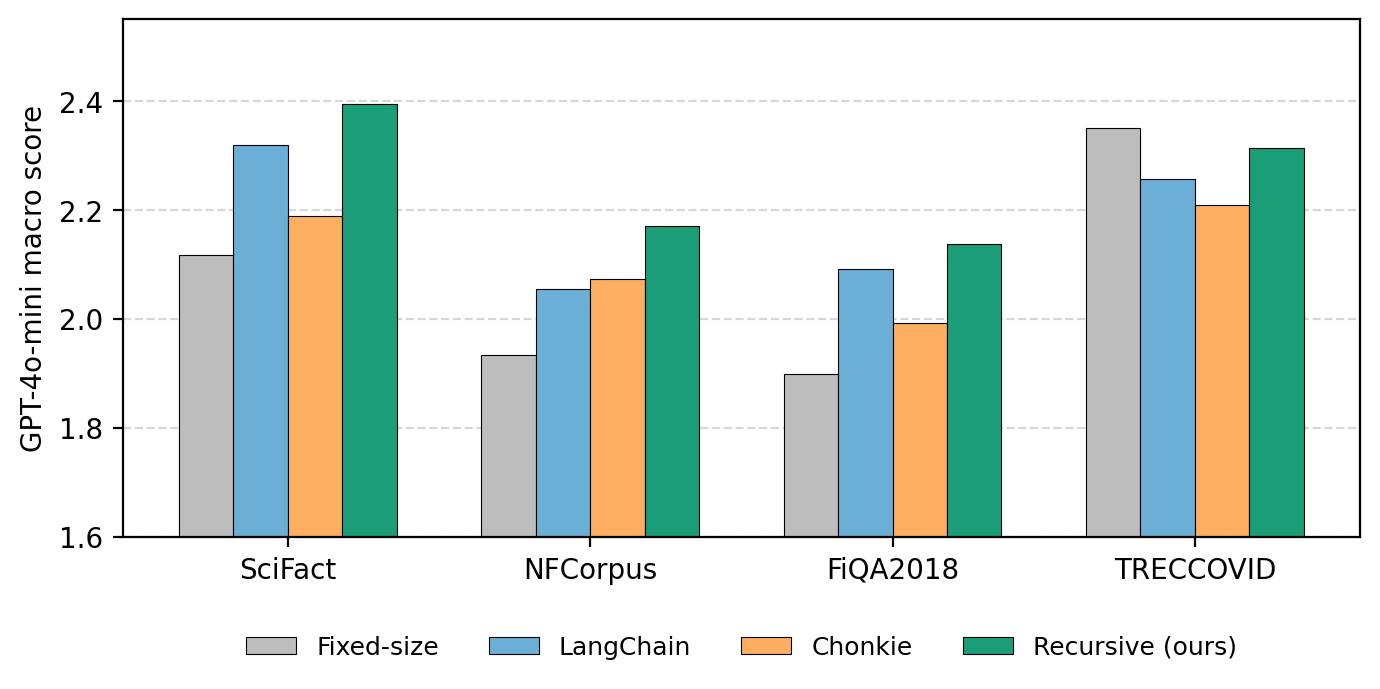
\includegraphics[width=\columnwidth]{results/figures/llm_judge_bars.png}
\caption{Macro-averaged GPT-4o-mini intrinsic scores (Coherence + Completeness + Relevance Purity, $0$--$3$ scale) by chunking method and dataset. Recursive chunking is the strongest method on three of four datasets; fixed-size chunking wins on TREC-COVID.}
\label{fig:llm_judge_bars}
\end{figure}

Figure~\ref{fig:correlation_scatter} pairs the GPT-4o-mini macro score with nDCG@10 from Table~\ref{tab:mteb_results}, averaged across the four embedding models. Pearson $r=0.85$ over $n{=}12$ paired cells (four datasets $\times$ three methods reported in both tables). The correlation supports using the intrinsic protocol as a screening signal prior to a full retrieval evaluation, complementary to but not redundant with retrieval metrics.

\begin{figure}[t]
\centering
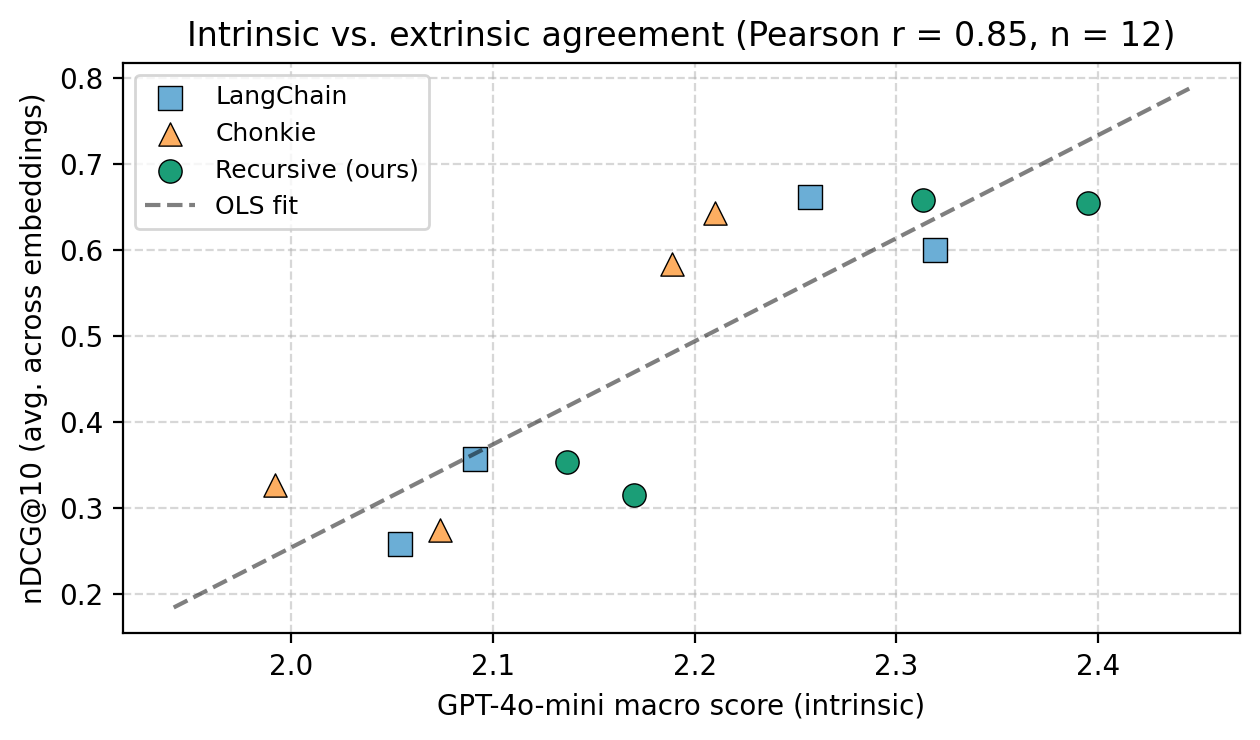
\includegraphics[width=\columnwidth]{results/figures/intrinsic_vs_extrinsic.png}
\caption{Intrinsic vs.\ extrinsic agreement. Each marker is a (dataset, method) cell; the $y$-coordinate is nDCG@10 averaged across the four MTEB embedding models from Table~\ref{tab:mteb_results}. Pearson $r=0.85$ across $n{=}12$ paired cells, indicating that GPT-4o-mini intrinsic scores meaningfully track retrieval quality.}
\label{fig:correlation_scatter}
\end{figure}

\subsection{Discussion}
Three patterns recur across the extrinsic and intrinsic results. (i) Recursive chunking is consistently strong on SciFact under both retrieval metrics and GPT-4o-mini scoring. (ii) Performance varies across embedding models in Table~\ref{tab:mteb_results}, so chunking quality cannot be studied independently of representation quality. (iii) Late Chunking shows consistent gains over naive chunking across datasets and boundary strategies, indicating that embedding-side improvements yield reliable retrieval gains under fixed boundaries.

\subsection{Error Analysis}
We classify chunking failures by their effect on retrieval. Three modes recur: (M1) an evidence span is split across chunks, reducing Recall@K; (M2) a short passage is over-segmented into low-context fragments with reduced embedding similarity to queries; (M3) a long passage is under-segmented into topically mixed chunks whose embeddings are noisy averages. The intrinsic axes localize these modes: Completeness penalizes M1 and M2; Relevance Purity penalizes M3. M2 dominates fixed-size failures on NFCorpus, where documents are short and technical. M3 dominates on FiQA2018, where documents are conversational and digressive. Recursive chunking reduces M2 and M3 because its boundary-strength score is sensitive to local discontinuities, but it does not eliminate M1 on dense scientific abstracts, where evidence spans can themselves contain strong internal discontinuities.

\section{Limitations}
\label{sec:limitations}

\textbf{Single judge model.} All intrinsic scores come from a single judge (\texttt{gpt-4o-mini}). LLM-as-a-Judge scores inherit length, position, verbosity, and style biases of the underlying model~\cite{tan2024judgebench,liu2025consjudge}. Inter-judge agreement is not measured. Replicating with a second judge (e.g., GPT-4.1, Claude Opus 4, Gemini 2.5 Pro, Qwen2.5-72B) and reporting Cohen's $\kappa$ would address this directly.

\textbf{Embedding-model coverage.} The extrinsic evaluation uses four small-to-medium open-weight embedding models; Late Chunking uses a different family (jina-v2-small, jina-v3, nomic-v1), so the cross-table comparison is qualitative. Larger commercial models (\texttt{text-embedding-3-large}, Voyage-3, Cohere v3) are not evaluated.

\textbf{Dataset coverage.} The four BEIR corpora consist of relatively short documents (scientific abstracts, FAQ passages, news-style medical content). Long-form, multi-section corpora (HiCBench~\cite{lu2025hichunk}, MS MARCO long passages, technical reports) are absent, despite being the regime where boundary quality is expected to matter most.

\textbf{Method coverage.} The dynamic programming method in Section~\ref{sec:method_dp} is deprioritized on compute grounds. CrossFormer, S2 Chunking, HiChunk, and HOPE are discussed but not run end-to-end, primarily because of their labeled-data and compute requirements.

\textbf{Axis independence.} The three intrinsic axes are correlated in practice; the macro-average therefore overstates effective precision. A factor analysis over a larger judged sample is required to characterize axis independence.

\section{Future Work}
Three extensions follow from the limitations above. (i) Replicating the intrinsic protocol with a second judge and reporting Cohen's $\kappa$. (ii) Combining recursive boundary selection with Late Chunking-style pooled embeddings to test whether the two levers compound. (iii) Evaluating on long-form corpora such as HiCBench~\cite{lu2025hichunk}.

A separate question concerns embedding construction. Some encoders expose token-level representations that admit mean pooling over span boundaries without re-encoding (as in Late Chunking); others require chunk-level recomputation. A direct comparison of pooled-span embeddings against natively re-encoded chunk embeddings, holding boundaries fixed, would isolate this effect.



\section{Code and Data}
The recursive chunker, the MTEB retrieval harness, the LLM-as-a-Judge runner, the five Jinja2 prompt templates, the result CSVs, and the figure-generation script are released at:

\begin{sloppypar}
\url{https://github.com/shellyganga/deep_learning_proj}
\end{sloppypar}

\section{Author Contributions}
Shelly Schwartz designed the methods and evaluation, implemented the recursive chunker and the LLM-as-a-Judge protocol, and conducted all experiments.

\section{Conclusion}
Boundary selection and embedding construction are complementary levers in chunking: improvements on one do not preclude improvements on the other. The marginal value of semantic boundary selection is, however, structure-dependent. It dominates on heterogeneous corpora (SciFact, NFCorpus, FiQA2018) but shrinks on the short, topically uniform abstracts of TREC-COVID, where fixed-size chunking wins intrinsically and the recursive method splits the extrinsic cells with LangChain. The Pearson $r=0.85$ agreement between the LLM-judge protocol and BEIR nDCG@10 supports its use as a low-cost diagnostic prior to retrieval evaluation.

\bibliographystyle{IEEEtran}
\bibliography{refs}

\appendix

\section{Appendix}
\label{sec:appendix}
This appendix provides the verbatim prompt templates used for the intrinsic LLM-as-a-Judge protocol and additional implementation details for reproducibility.

\subsection{Implementation}
Each prompt is rendered from a Jinja2 template at evaluation time and submitted to the judge through a single LLM gateway call. The judge response is parsed as a single integer in $[0,3]$ and aggregated into per-axis means and a macro-average. The judge is GPT-4o-mini with temperature $0$, top-$p$ $1$, and a $4$-token output cap.

\section{Prompt Templates}
The five templates used in this paper are reproduced verbatim below. All request a single integer in the $0$--$3$ range and are used at temperature $0$. They fall into three groups: (i) a boundary-pair scorer that presents two adjacent chunks and asks whether the cut between them is well placed; (ii) a self-segment scorer that presents a single passage and asks whether it should be split further; and (iii) the three axis-based intrinsic scorers used for Table~\ref{tab:llm_judge_results}.

\subsection{Boundary-Pair Scorer}

\begin{promptbox}{Boundary-pair scorer}
\begin{lstlisting}
You are an expert text segmentation evaluator.
You are given a piece of text, split into two parts: PART 1 and PART 2.
Evaluate how optimally the split location was chosen, i.e.,
how much the two parts are logically and semantically independent.

Output only a single digit between 0 and 3 with no explanation.

Scoring rubric:
0 - Very not optimal: a split almost anywhere would result in the same or better separation.
1 - Poorly optimal: many other places would yield better separation.
2 - Moderately optimal: only a few other places would yield better separation.
3 - Highly optimal: almost no other place would yield better separation.

PART 1:
{{ part1 }}

PART 2:
{{ part2 }}
\end{lstlisting}
\end{promptbox}

\subsection{Self-Segment Scorer}

\begin{promptbox}{Self-segment scorer}
\begin{lstlisting}
You are an expert in judging a chunking of a text for purposes of RAG.
You examine a text and assess whether it is uniform and compact enough to be
a single chunk, or the text can be split into two or more chunks.

You output only a single score which is a number between 0 and 3.
0 - No split needed: The text is the best as a single chunk.
1 - Possible, but not necessary.
2 - Possible good split.
3 - Split is necessary.

{{ text }}
\end{lstlisting}
\end{promptbox}

\subsection{Axis-Based Intrinsic Scorers}

\begin{promptbox}{Coherence}
\begin{lstlisting}
You are an expert evaluator of text segmentation for retrieval-augmented
generation (RAG). You are given a chunked document. The chunks are listed
below in order, separated by the marker [CHUNK BREAK]. Each [CHUNK BREAK]
represents a proposed split point chosen by a chunking algorithm.

Your task is to evaluate the COHERENCE of the chunking, i.e., whether
the proposed split points correctly divide the text at semantically
independent boundaries, so that adjacent chunks discuss distinct ideas
rather than artificially fragmenting a single idea across a boundary.

Output only a single integer between 0 and 3, with no explanation.

Scoring rubric:
0 - Incoherent: most splits cut through the middle of a single idea.
1 - Weakly coherent: several splits fall in the middle of an idea.
2 - Mostly coherent: most splits fall at reasonable semantic transitions.
3 - Highly coherent: nearly every split aligns with a clear semantic transition.

CHUNKED DOCUMENT:
{{ chunked_text }}
\end{lstlisting}
\end{promptbox}

\begin{promptbox}{Completeness}
\begin{lstlisting}
You are an expert evaluator of text segmentation for retrieval-augmented
generation (RAG). You are given a single chunk produced by a chunking
algorithm. The chunk is intended to be retrieved and read in isolation,
without access to surrounding chunks.

Your task is to evaluate the COMPLETENESS of the chunk, i.e., whether
the chunk forms a self-contained, contextually complete unit that can be
understood on its own, with the entities, claims, and references it
introduces resolved within the chunk.

Output only a single integer between 0 and 3, with no explanation.

Scoring rubric:
0 - Severely incomplete: relies heavily on missing context.
1 - Partially incomplete: several unresolved references or claims.
2 - Mostly complete: largely self-contained with minor unresolved references.
3 - Fully complete: every introduced entity and reference is resolved.

CHUNK:
{{ chunk }}
\end{lstlisting}
\end{promptbox}

\begin{promptbox}{Relevance Purity}
\begin{lstlisting}
You are an expert evaluator of text segmentation for retrieval-augmented
generation (RAG). You are given a single chunk produced by a chunking
algorithm.

Your task is to evaluate the RELEVANCE PURITY of the chunk, i.e.,
whether the content within the chunk maintains a single, consistent
topic without mixing unrelated information. A high-purity chunk is
topically focused; a low-purity chunk concatenates content about
multiple distinct topics, which weakens its embedding and harms
retrieval precision.

Output only a single integer between 0 and 3, with no explanation.

Scoring rubric:
0 - Impure: mixes two or more unrelated topics with no shared thread.
1 - Weakly pure: loosely related, spans multiple distinct subtopics.
2 - Mostly pure: largely focused on one topic with minor drift.
3 - Highly pure: a single, consistent topic throughout.

CHUNK:
{{ chunk }}
\end{lstlisting}
\end{promptbox}

\end{document}
